\documentclass[a4paper,10pt]{article}
\usepackage{url}
\usepackage{graphicx}
\usepackage[utf8]{inputenc}
\usepackage[backend=biber,autocite=footnote,notetype=foot+end,style=authortitle-ibid]{biblatex}
\bibliography{group4}

\begin{document}

    \title{Sentiment Analysis of Twitter Data based on Implicit Categories in Textual Weather Data}
    \author{
        Johnston, Cian
        \and
        Ravindran, Aishwarya
        \and
        Chavady, George
        \and
        Karode, Sameer
        \and
        Kulkarni, Shravani Deepak
    }

    \maketitle
    \section{Introduction}

    Sentimental mining is a critical and essential area because sentiment fundamentally relates to a person’s emotions, impression and attitude. Analysing every individual’s sentiments from a text analytics point of view accurately is challenging. We are basically trying to comprehend the thoughts and assumptions of an individual regarding a concept or topic with some context be it positive, negative or neutral \footfullcite{aylien_sentiment}. It is estimated that nearly 2.5 Quintillion bytes of data is generated each day \footfullcite{blazon_howmuchdata} and there is a plethora of information relating to a person’s messages, tweets, documents, emails, chats, conversations and comments available. Sentiment analysis aids us in analysing this huge amount of data efficiently.

    In this paper, we focus on performing sentiment analysis on the weather based on data retrieved from Twitter \footfullcite{mining_twitter_data}. Twitter, being an acclaimed stage for social networking possess and people to express their interests and thoughts has plenty of information from posts known as “tweets”. With over 500 million tweets per day pertaining to almost anything, it is an excellent platform due to its accessibility and real-time analysis of the data which is crucial for sentiment analysis. It is not uncommon that weather plays an important role in an individual’s mood and its consequences because of the decisions made. 
    
    In this paper, we present an analysis of tweets for the year 2018 in the geographical area of Ireland. At a broader level, we analyze the tweets season-wise to understand the general sentiment in the tweets for each of the four seasons that are experienced in Ireland (winter, spring, summer and autumn). For instance, we compare the emotions in the tweets in summer vs the tweets in winter. Additionally, at a deeper level, we analyze the tweets for each day and correlate it with the weather on that day. In this case, we find the trends in the sentiments on sunny, cloudy, wet, dry or cold days. Furthermore, we also compare these trends on weekdays and weekends. For these analysis, we make use of visualizations to gain more insights into finding patterns between the weather and sentiment of the population within a given geographical region.


    \section{Related Work}

    As the accessibility to real-time information or otherwise is increasing, performing analysis on this data is also becoming viable. There has been a lot of notable research done on sentiment analysis of twitter data in general and studies emphasizing on correlating weather with people’s mood and sentiments from Twitter data by measuring temperature, humidity and atmospheric pressure \footfullcite{park2013mood}. These weather variables seem to have a satisfactory impact on one’s mood. Another paper \footfullcite{bagheri2017sentiment} focuses on implementing sentiment analysis on Twitter data using the Twitter API’s and a wealth of available libraries. Twitter is known for having small texts and abbreviations used by people in their posts or tweets making it challenging to extract polarity of the texts and hence researchers resort to utilizing deep learning and machine learning techniques.
    
    Researchers have performed sentiment analysis for various reasons and different areas like elections, politics, movie ratings and fashion to name a few. In 2015, there was a noteworthy research done in the vision of predicting future crime on each area of a major city, Chicago, Illinois of the United States using GPS tagged twitter data \footfullcite{chen2015crime}. They aimed to predict the time and location during which a specific type of crime is expected to occur by applying lexicon-based sentiment analysis on categorized weather data combined with kernel density estimation of historical crime incidents and were successful. Hannak et al. \footfullcite{hannak2012tweetin} concentrate on using a Twitter specific sentiment extraction methodology and explore a corpus of over 1.5 billion tweets. With the help of machine learning techniques on Twitter corpus correlated with the weather at a particular time and location of the tweets, it was concluded that aggregate sentiment follows different climate and seasonal patterns.

    \section{Methodology}

    Our hypothesis is that there exists a significant correlation between the overall sentiment of Tweets at a given time, and the features of a given weather forecast for the same specified time on which that Tweet was posted. The null hypothesis is that no significant correlation exists. In order to address the hypothesis, two sources of data were procured: a collection of posts from Twitter, and a collection of textual weather data. Both of these corpora were assembled and filtered such that they both relate to the same geographical area, and to the same timespan. The geographical area in question was restricted to the Republic of Ireland, and the timespan in question was limited to the year of 2018. 

    \subsection{Twitter Data}

    \subsubsection{What to measure}

    To measure the sentiment of a Tweet, we elected to use the \texttt{TextBlob} \footfullcite{textblob_doc} library, which internally utilises a Naive Bayes classifier pre-trained on a corpus of movie reviews. Applying this classifier to a text yields a tuple of two real-valued integers in the range [-1.0, 1.0], denoting both the \textit{polarity} and the \textit{subjectivity} of the text.

    \subsubsection{Data Collection}

    Twitter provides an API for developers to both read data and interact with users. This has a number of limitations, including rate limits \footfullcite{twitter_api_docs_rate_limit}, and a requirement to request an API key. In order to access a useful volume of data, this would require a large number of HTTP requests to Twitter. Thankfully, the Internet Archive provides a large dataset of posts on Twitter for the year of 2018 in TAR format \footfullcite{archiveorg_twitter}. While these datasets are essentially a subset of the \textit{global} content of Twitter, and technically much larger than required, they are hosted using BitTorrent and are thus much more straightforward to download. For the purposes of this paper, we elected to use a subset of the Twitter archive data from the year 2018.

    \subsubsection{Data Processing}

    The large archives detailed above needed to be preprocessed before any meaningful analysis can be performed. To this end, a small program was written to consume the entire TAR archive and filter out Tweets matching certain criteria, serializing a subset of the data to CSV format. This was done to avoid extracting the entire archive to disk, which is a time-consuming operation. The following criteria were used for extracting Tweets of interest:
    \begin{itemize}
        \item{
            Having geo-location information within Ireland, or
        }
        \item{
            Posted by a user with user-specified location containing the string \textit{Ireland}.
        }
    \end{itemize}

    Note that not all Tweets posted by users in Ireland will necessarily have geo-location information attached, and not all Tweets posted by users claiming to be located within Ireland are necessarily so.

    \subsubsection{Data Cleaning}

    The tweets are 140 characters long. Considering this constraint, initial analysis from the chunk of tweets revealed that, users tend to use more contractions and emojis to express their thoughts rather than using appropriate grammar. The sentiment score given by the existing implementations like TextBlob is affected by the use of such text. We implemented a python code to do the preprocessing of the data obtained, which is obtained using Twitter API.

    The filtering process removes the URLs, usernames, and hashtags. In some situations, it is known that hashtags can provide instant insight as to what the users are feeling. However, most hashtags that we encountered contain meaningless text or sentences for tags instead of keywords. The process flow is illustrated in Figure \ref{fig:twitter_process_flow}.

    \begin{figure}
        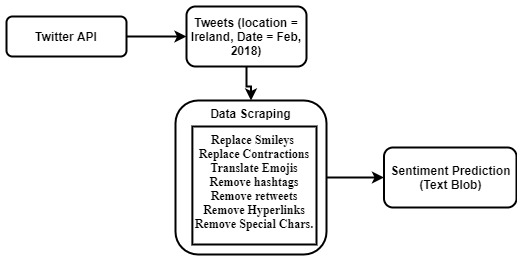
\includegraphics[width=0.8\textwidth]{twitter_process_flow.jpeg}
        \caption{Twitter data process flow.}
        \label{fig:twitter_process_flow}
    \end{figure}

    \begin{itemize}
        \item{
            We removed hashtags, retweets, @mentions, hyperlinks and special characters using regular expressions.
            \\ \\
            \textit{for example, \\  }
            {\textbf{Sample Input: \\} \textit{ Hello there, This is sample tweet with mentions@john, \#hashtag and link https://google.com} \\ }
            {\textbf{Processed Output: \\}\textit{  Hello there, This is sample tweet with mentions, hashtag and link \\ } }
        }
        \item{
            Next, we replaced all the contractions in the tweets to its original forms. We used a dictionary of all the contractions with its original form and replaced them in the text.
            \\ \\
            \textit{for example, \\  }
            {\textbf{Sample Input: \\} \textit{Hello, how're you doing?} \\ }
            {\textbf{Processed Output: \\}\textit{   Hello, how are you doing? \\ } }
        }
        \item{
            Lastly, we translated all the emojis/smileys to texts. For the smileys using special characters, we used the same approach as in the previous step (a dictionary containing the smileys and their corresponding meaning). We utilized the emoji library available in python for this conversion.
            \\ \\
            \textit{for example, \\  }
            {\textbf{Sample Input: \\} \textit{ Sample tweet with :-) and <3 } \\ }
            {\textbf{Processed Output: \\}\textit{   Sample tweet with happy smiley and love \\} }
        }\end{itemize}



    \subsection{Weather Data}

    \subsubsection{What to measure}

    For the purposes of this hypothesis, given a textual weather forecast and a finite set of potential features of weather forecasts, we map each textual forecast to a subset of those potential features. The features of each individual forecast text are determined by the presence or absence of a set of manually selected tokens.

    \subsubsection{Data Collection}

    Some historical weather data was collected from MET \'{E}ireann, the Irish National Meteorological Service. \footfullcite{metie}. Unfortunately, historical textual weather forecast data is not available from MET \'{E}ireann; to work around this, we used the Internet Archive's Wayback Machine \footfullcite{wayback_machine} to access previously published versions of the MET \'{E}ireann homepage which contains daily textual forecast data.

    To access previously versions of the website more conveniently, the tool \texttt{wayback-machine-scraper} was utilised \footfullcite{github_sangaline_wayback-machine-scraper}. This is a command-line utility that interfaces with \textit{Wayback Machine} and allows a user to download a number of snapshots of a website for a specified date range. For the purposes of this paper, we fetched all the saved snapshots of the MET \'{E}ireann homepage for the year of 2018. Note that this is a sparse dataset, and snapshots of this data is not available for every day.

    As an alternative source of textual forecast data, we turned to a more unorthodox source -- Boards.ie is a discussion board with a wide range of fora which, naturally, includes the topic of weather. One particular thread of interest on this sub-forum has almost daily forecasts provided by an amateur meteorologist with the moniker 'M.T. Cranium' \footfullcite{boards_ie_mt_cranium_forecasts}. The relevant print versions of the thread spanning the year of 2018 were saved, and the relevant daily forecasts were extracted using a Python script. The process is illustrated below in Figure \ref{fig:weather_process_flow}.

    \begin{figure}
        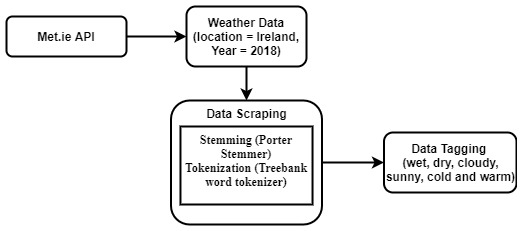
\includegraphics[width=0.8\textwidth]{weather_process_flow.jpeg}
        \caption{Weather data process flow.}
        \label{fig:weather_process_flow}
    \end{figure}


    \subsubsection{Data Processing}

    The textual forecast data on its own needs to be processed before any meaningful correlations can take place. To this end, we utilised the Python NLTK libraries to perform the following:
    \begin{itemize}
        \item{
            Stemming and tokenization of the raw text. NLTK provides pre-implemented stemmers and tokenizers for the English language. For stemming we utilised a \texttt{PorterStemmer} \footfullcite{nltk_doc_stem_porter}, and for tokenization, a \texttt{TreebankWordTokenizer} \footfullcite{nltk_doc_tokenize_treebank}. \\
            For example, the raw string \texttt{``TODAY ... Continued mild with a few outbreaks of light rain, highs near 12 C.''}, after stemming and tokenization, becomes a list of tokens \texttt{[ `today', `...', `continu', `mild', `with', `a', `few', `outbreak', `of', `light', `rain', `,' ,`high', `near', `12', `c', `.' ]}.
        }
        \item{
            Annotation of the tokenized forecast data with some predefined features. For an initial first pass, we defined a na\"{i}ve approach whereby a number of binary features were defined: \textit{wet, dry, cloudy, sunny, cold, warm}. For each feature, a number of tokens were selected to signify if the feature should be 1, and 0 otherwise. For example, the presence of the token \textit{rain} in the forecast signifies a value of 1 for the feature \textit{wet}. These features were then extracted for all of the collected forecast data and serialized to CSV format.
        }
    \end{itemize}

	\subsection{Sentiment Analysis}
	
	After preprocessing of the tweet corpus, the same is processed for carrying out the sentiment analysis. Initially, the text corpus is processed using TextBlob, which is a python library built over Natural Language Toolkit(NLTK). TextBlob provides a sufficient set of tools for performing tasks like Sentiment Extraction, Spelling Correction and Detection of Language. There are two types of sentiment analyzers, by default, the TextBlob uses PatternAnalyzer and second is NaiveBayesAnalyzer. The next steps are to evaluate the sentiment score given by the default and overridden implementation of Analyzer. Once the tweets are labelled with its sentiment score, the analysis is done to find correlations between weather data and sentiment score of tweets. The weather data is classified into categories for analysis. 


    \section{Results}

    The findings of our initial analysis of sentiment in Twitter data were that there were more tweets that showed positive sentiment than tweets that displayed negative sentiment.

    \section{Future Work}  
    Our future work would involve collecting Twitter data posted during different seasons of the year. More specifically, when the weather data collected is disparate. This data would help us in gauaging the effects of weather on Twitter posts.  For example, an increase in temperature from lower values to values between 15C and 20C are associated with significant increases in positve expressions. On the contrary, the number of expressions of positive sentiment decline when the temperature exceeds a value of 30C. 


    \section{Conclusion}

     Large amounts of data is readily available on Twitter which can be used to analyze sentiment of the users' tweets. Also, historical and real time weather data is made available by the meteorogical department. We could use weather data and analyze it together with the tweets to predict sentiment for a particular weather forecast using Machine Learning algorithms. Studies have shown that weather conditions such as temperature, precipitation, cloud cover, wind speed and humidity each significantly relate to the expression of sentiment in social media such as Twitter and Facebook. Analysis of sentiment correlated with weather data gives us some important background information of the users of the system.

\end{document}
